\documentclass{article}

\usepackage[final]{iai_neurips_2024}
\usepackage{makecell}
\bibliographystyle{unsrtnat}
\usepackage[english]{babel}
\usepackage[utf8]{inputenc}
\usepackage{graphicx} 
\usepackage{booktabs} 
\usepackage{algorithm}
\usepackage{framed}
\usepackage{tikz-cd}
%\usepackage{adjustbox}
%\usepackage{pst-node, auto-pst-pdf}


\usepackage[backslant]{aurical}       % Fontauri fonts 
\usepackage{bm}
\usepackage[utf8]{inputenc} % allow utf-8 input
%\usepackage[T1]{fontenc}    % use 8-bit T1 fonts
\usepackage{hyperref}       % hyperlinks
\usepackage{url}            % simple URL typesetting
\usepackage{booktabs}       % professional-quality tables
\usepackage{amsfonts}       % blackboard math symbols
\usepackage{nicefrac}       % compact symbols for 1/2, etc.
\usepackage{microtype}      % microtypography
\usepackage{subfig}
\usepackage{tabularx}
\usepackage{amsmath}
\usepackage{enumerate}
\usepackage{xcolor}
\usepackage[font=small]{caption}
%\usepackage[labelformat = empty,position=top]{subcaption}
\usepackage[export]{adjustbox}
%\usepackage{subcaption}

\usepackage[backend=biber,style=apa,sorting=ynt]{biblatex}

% \bibliographystyle{plainnat}

\usepackage{float}
\usepackage{placeins}
\usepackage{multirow}
\usepackage{mdframed}
\usepackage{media9}

\captionsetup[algorithm]{labelformat=empty}
% \usepackage{algpseudocode}
\usepackage{algorithmic}

\newcommand{\ols}{\textsc{ols}}


\newenvironment{itemize*}{
\begin{itemize}
\setlength{\parskip}{0em}
\setlength{\topparskip}{0em}
}
{\end{itemize}}

\newenvironment{enumerate*}{
\begin{enumerate}
\setlength{\parskip}{0em}
\setlength{\topparskip}{0em}
}
{\end{enumerate}}


% Commands
\newcommand{\comment}[1]{}
\newcommand{\techreport}[1]{#1}

\newcommand{\beq}{\begin{equation}}
\newcommand{\eeq}{\end{equation}}
\newcommand{\beqa}{\begin{eqnarray}}
\newcommand{\eeqa}{\end{eqnarray}}
\newcommand{\beqas}{\begin{eqnarray*}}
\newcommand{\eeqas}{\end{eqnarray*}}

\newcommand{\bit}{\begin{itemize}}
\newcommand{\eit}{\end{itemize}}
\newcommand{\bits}{\begin{itemize*}}
\newcommand{\eits}{\end{itemize*}}
\newcommand{\benum}{\begin{enumerate}}
\newcommand{\eenum}{\end{enumerate}}
\newcommand{\benums}{\begin{enumerate*}}
\newcommand{\eenums}{\end{enumerate*}}
\newcommand{\mybullet}{$\bullet$}

%\newcommand{\BlackBox}{\rule{1.5ex}{1.5ex}}  % end of proof

% names

\newcommand{\dpullalg}{{\sc PullBackDPhi}}
\newcommand{\projg}{{\sc ProjectG}}
\newcommand{\glassoalg}{{\sc GroupLasso}}
\newcommand{\embedalg}{{\sc EmbeddingAlg}}
\newcommand{\flassoalg}{{\sc GroupLasso}}
\newcommand{\flasso}{{\sc GroupLasso}}  % to be replaced with \flassoalg !!
\newcommand{\LEalg}{{\sc LaplacianEigenmaps}}
\newcommand{\rmalg}{{\sc RMetric}}
\newcommand{\lapalg}{{\sc Laplacian}}
\newcommand{\tppalg}{{\sc LocalPCA}}
\newcommand{\ouralg}{{\sc ManifoldLasso}}


\newcommand{\srdata}{{\bf SwissRoll}}
\newcommand{\redata}{{\bf RigidEthanol}}
\newcommand{\ethdata}{{\bf Ethanol}}
\newcommand{\toldata}{{\bf Toulene}}
\newcommand{\maldata}{{\bf Malonaldehyde}}

%  math mode commands

\newcommand {\argmax}[2]{\mbox{\raisebox{-1.7ex}{$\stackrel{\textstyle
 {\rm #1}}{\scriptstyle #2}$}}\,}
\newcommand{\nchoosem}[2]{\left(\!\!\!\begin{array}{c}#1\\#2\end{array}\!\!\!\right)}  % use \binom{}{} instead
\newcommand{\fracpartial}[2]{\frac{\partial #1}{\partial  #2}}

\newcommand{\bigOO}{{\cal O}}
\newcommand{\dataset}{{\cal D}}
\newcommand{\onevector}{{\mathbf 1}}
\newcommand{\rrr}{{\mathbb R}}

\newcommand{\M}{{\cal M}}
\newcommand{\T}{{\cal T}}
\newcommand{\txim}{\ensuremath{\T_{\xi_i}\M}} % tangent subspace
\newcommand{\I}{{\cal I}} % set of indices for which to compute gradients

\newcommand{\G}{{\cal G}} % dictionary
\newcommand{\neigh}{{\cal N}}
\newcommand{\X}{{\cal X}}
\newcommand{\xb}{\mathbf{X}}  % matrices for glasso
\newcommand{\tilx}{\tilde{x}}
%\newcommand{\g}{\Fontauri{g}} % R metric as a form Fontauri not working!
\newcommand{\g}{\mathbf{g}} % R metric as a form
%\newcommand{\id}{\Fontauri{id}} % induced Euclidean metric as a form
\newcommand{\id}{\mathbf{id}} % induced Euclidean metric as a form


\newcommand{\proj}{\operatorname{Proj}}
\newcommand{\trace}{\operatorname{trace}}
\newcommand{\rank}{\operatorname{rank}}
\newcommand{\range}{\operatorname{span}}
\newcommand{\rowrange}{\operatorname{rowspan}}
\newcommand{\diag}{\operatorname{diag}}
\newcommand{\grad}{\operatorname{grad}}
\newcommand{\supp}{\operatorname{supp}}

\newcommand{\barbx}{\bar{\bar{X}}}
\newcommand{\bhat}{\hat{\beta}}
\newcommand{\zhat}{\hat{z}}
\newcommand{\barw}{\bar{\epsilon}}
\newcommand{\bbar}{\bar{\beta}}

\newcommand{\E}{{\cal E}} %the error manifold
\newcommand{\N}{{\cal N}} %a normal space
\newcommand{\Ho}{{\cal H}} %the horizontal space of a map
\newcommand{\V}{{\cal V}} %the vertical space of a map
\newcommand{\B}{{\cal B}} %the base manifold
\newcommand{\txm}{\ensuremath{\T_{\xi}\M}}
\newcommand{\tbasis}{\mathbf{T}} % basis T
\newcommand{\cp}{\text{cp}}
\newcommand{\tstsbp}{{\sc TwoStageTSBP}}
\newcommand{\tsalg}{{\sc TSLasso}}
\newcommand{\tsbp}{{\sc TSBasisPursuit}}
\newcommand{\embedts}{\textsc{EmbedTS}}
\newcommand{\embedgrad}{{\sc EmbedGrad}}
\captionsetup[algorithm]{labelformat=empty}
\newtheorem{proposition}{Proposition}


\tikzset{%
  symbol/.style={
    draw=none,
    every to/.append style={
      edge node={node [sloped, allow upside down, auto=false]{$#1$}}
    },
  },
}

\usepackage{tcolorbox}

\tcbuselibrary{fitting}

\newenvironment{proof}{\paragraph{Proof:}}{\hfill$\square$}


\newcommand{\M}{\mathcal{M}}
\newcommand{\N}{\mathcal{N}}


\title{Isometry pursuit}

\author{%
  Samson Koelle \\
  Amazon  \\
  koelle@amazon.com
  \And
  Marina Meila \\
  Department of Statistics\\
  University of Washington \\
  mmp@uw.edu
}

\begin{document}

\maketitle

\begin{abstract}
Isometry pursuit is a convex algorithm for identifying orthonormal column-submatrices of wide matrices.
It consists of a novel normalization method followed by multitask basis pursuit.
Applied to Jacobians of putative coordinate functions, it helps identity isometric embeddings from within interpretable dictionaries.
We provide theoretical and experimental results justifying this method.
For problems involving coordinate selection and diversification, it offers a synergistic alternative to greedy and brute force search.
\end{abstract}

\footnotetext[1]{Work conducted outside of Amazon.}

\section{Introduction}
\label{sec:introduction}

Many real-world problems may be abstracted as selecting a subset of the columns of a matrix representing stochastic observations or analytically exact data.
This paper focuses on a simple such problem that appears in interpretable learning and diversification.
Given a rank $D$ matrix $ X \in \mathbb R^{D \times P}$ with $P > D$, select a square submatrix $ X_{.\mathcal S}$ where subset $ S \subset P$ satisfies $| S| = D$ that is as orthonormal as possible.

This problem arises in interpretable learning specifically because while the coordinate functions of a learned latent space may have no intrinsic meaning, it is sometimes possible to generate a dictionary of interpretable features which may be considered as potential parametrizing coordinates.
When this is the case, selection of candidate interpretable features as coordinates can take the above form.
While implementations vary across data and algorithmic domains, identification of such coordinates generally aids mechanistic understanding, generative control, and statistical efficiency.

This paper shows that an adapted version of the algorithm in \citet{Koelle2024-no} leads to a convex procedure that can improve upon greedy approaches such as those in \citet{5895106, NEURIPS2019_6a10bbd4, Kohli2021-lr, Jones2007-uc} for finding isometries.
The insight leading to isometry pursuit is that multitask basis pursuit applied to an appropriately normalized $ X$ selects orthonormal submatrices.
Given vectors in $\mathbb R^D$, the normalization log-symmetrizes length and favors those closer to unit length, while basis pursuit favors those which are orthogonal.
Our results formalize this intuition within a limited setting, and show the usefulness of isometry pursuit as a trimming procedure prior to brute force search for diversification and interpretable coordinate selection.
We also introduce a novel ground truth objective function to measure the success of our algorithm against, and discuss the reasonableness of this trimming procedure.

 \footnotetext[2]{Code is available at \url{https://github.com/sjkoelle/isometry-pursuit}.}
\section{Background}

Our algorithm is motivated by spectral and convex analysis.

\subsection{Problem}

Our goal is, given a matrix $ X \in \mathbb R^{D \times P}$, to select a subset $ S \subset [P]$ with $| S| = D$ such that $X_{.  S}$ is as orthonormal as possible in a computationally efficient way.
To this end, we define a ground truth loss function that measures orthonormalness, and then introduce a surrogate loss function that convexifies the problem so that it may be efficiently solved.
Figure \ref{fig:data} and \ref{fig:selection} provide a visual depiction of this problem when $D=2$ and $P=30$.

\subsection{Interpretability and isometry}

Our motivating example is the selection of data representations from within sets of putative coordinates: the columns of a provided wide matrix.
Compared with Sparse PCA \citep{DAspremont2007-aq, Dey2017-mx, Bertsimas2022-qo, Bertsimas2022-dv}, we seek a low-dimensional representation from the set of these column vectors rather than their span.

This method applies to interpretability, for which parsimony is at a premium.
Interpretability arises through comparison of data with what is known to be important in the domain of the problem.
This knowledge often takes the form of a functional dictionary.
Evaluation of independence of dictionary features arises in numerous scenarios \citep{Chen2019-km, Koelle2022-ju, He2023-ch}.
The requirement that dictionary features be full rank has been called functional independence \citep{Koelle2022-ju} or feature decomposability \citep{templeton2024scaling}, with connection between dictionary rank and independence via the implicit function theorem.
Besides independence, the metric properties of such dictionary elements are of natural interest.
This is formalized through the notion of differential.

\begin{definition}
The \textbf{differential} of a smooth map $\phi:\mathcal M \to \mathcal N$ between $D$ dimensional manifolds $\M \subseteq \mathbb R^B$ and $\N \subseteq \mathbb R^P$ is a map in tangent bases $x_1 \dots x_{D}$ of $T_\xi \M$ and $y_1 \dots y_{D}$ of $T_{\phi(\xi)} \N$ consisting of entries
\begin{align}
\label{eq:diff}
    D\phi (\xi) = \begin{bmatrix}
    \frac{\partial \phi_1  }{\partial x_1}(\xi)  & \dots & \frac{\partial \phi_1 }{\partial x_D}(\xi)  \\
    \vdots & & \vdots \\
    \frac{\partial \phi_D }{\partial x_1}(\xi)  & \dots & \frac{\partial \phi_{D}  }{\partial x_{D}}(\xi) 
    \end{bmatrix}.
\end{align}
\end{definition}

It is not always necessary to explicitly estimate tangent spaces when applying this definition.
The most commonly encountered manifolds are vector spaces for which the tangent spaces are trivial.
This is the case for full-rank tabular data, for which isometry has a natural interpretation as a type of diversification, and often for the latent spaces of deep learning models.
In this case, $B = D$.

\begin{definition}
\label{def:isometric_at_a_point}
A map $\phi$ between $D$ dimensional submanifolds with inherited Euclidean metric $\mathcal M \subseteq R^{B}$ and $\mathcal N  \subseteq R^{P}$
$\phi$ is an \textbf{isometry at a point} $\xi \in \mathcal M$ if
\begin{align}
{D \phi (\xi)}^T D \phi (\xi) = I_D.
\end{align}
That is, $\phi$ is an isometry at $\xi$ if $D \phi (\xi)$ is orthonormal.
\end{definition}

The applications of pointwise isometry are themselves manifold.
Pointwise isometric embeddings faithfully preserve high-dimensional geometry.
For example, Local Tangent Space Alignment \citep{ZhangZ:04}, Multidimensional Scaling \citep{ChenBuja:localMDS09} and Isomap \citep{tenenbaum2000ggf} non-parametrically estimate embeddings that are as isometric as possible.
Another approach stitches together pointwise isometries selected from a dictionary to form global embeddings \citep{Kohli2021-lr}.
The method is particularly relevant since it constructs such isometries through greedy search, with putative dictionary features added one at a time.

That $D\phi$ is orthonormal has several equivalent formulations.
The one motivating our ground truth loss function comes from spectral analysis.
\begin{proposition}
\label{prop:orthonormal_spectrum}
The singular values $\sigma_1 \dots \sigma_D$ are equal to $1$ if and only if $U \in \mathbb{R}^{D \times D}$ is orthonormal.
\end{proposition}
On the other hand, the formulation that motivates our convex approach is that orthonormal matrices consist of $D$ coordinate features whose gradients are orthogonal and of unit length.
\begin{proposition}
\label{prop:orthonormal_basis}
The component vectors $u_1 \dots u_D \in \mathbb R^B$ form a orthonormal matrix if and only if, for all $d_1, d_2 \in [D], \langle u_{d_1}, u_{d_2} \rangle = \begin{cases}
1 \; d_1 = d_2 \\ 
0 \; d_1 \neq d_2 
\end{cases}$.
\end{proposition}


\subsection{Best subset selection}

Given a matrix $ X \in \mathbb R^{D \times P}$, we compare algorithmic paradigms for solving problems of the form
\begin{align}
\label{prog:ground_truth}
\arg \min_{ S \in \binom{[P]}{D}} l ( X_{. S})
\end{align}
where $\binom{[P]}{D} = \left\{ A \subseteq [P] : \left|A\right| = D \right\}$.
Brute force algorithms consider all possible solutions.
These algorithms are conceptually simple, but have the often prohibitive time complexity $O(C_lP^D)$ where $C_l$ is the cost of evaluating $l$.
Greedy algorithms consist of iteratively adding one element at a time to $ S$.
This algorithms have time complexity $O(C_lPD)$ and so are computationally more efficient than brute force algorithms, but can get stuck in local minima.
Formal definitions are given in Section \ref{sec:algorithms}.

Sometimes, it is possible to introduce an objective which convexifies problems of the above form  \citep{Liberti2004-iu, Abdi2013-th, Zhou2021-zz}.
Solutions
\begin{align}
\arg \min f(\beta) : Y  = X\beta 
\end{align}
to the overcomplete regression problem $Y = X \beta$ are a classic example \citep{Chen2001-hh}.
When $f(\beta) = \|\beta\|_0$, this problem is non-convex, and is thus suitable for greedy or brute algorithms, but when $f(\beta) =\|\beta\|_1$, the problem is convex, and may be solved efficiently via interior-point methods.
When the equality constraint is relaxed, Lagrangian duality may be used to reformulate as a so-called Lasso problem, which leads to an even richer set of optimization algorithms \citep{Hastie2016-cn}. % cite FISTA< glmnet, coordinate descent

The form of basis pursuit that we apply is inspired by the group basis pursuit approach in \citet{Koelle2022-ju}.
In group basis pursuit (which we call multitask basis pursuit when grouping is dependent only on the structure of matrix-valued response variable $y$) the objective function is $f(\beta) = \|\beta\|_{1,2} := \sum_{p=1}^P \|\beta_{p.}\|_2$  \citep{Yuan2006-bt, Obozinski2006-kq, Yeung2011-fg}.
This objective creates joint sparsity across entire rows $\beta_{p.}$ and was used in \citet{Koelle2022-ju} to select independent subsets among interpretable features.
\section{Method}

Recall that our objective is to, given a rank $D$ matrix $\mathcal X \in \mathbb R^{D \times P}$ with $P > D$, select a square submatrix $\mathcal X_{.\mathcal S}$ where subset $\mathcal S \subset P$ satisfies $|\mathcal S| = D$ that is as unitary as possible.
Thus, we first will define a function that is uniquely minimized by unitary matrices and some favorable properties for optimization that will be the ground truth we evaluate the success of our method against.
We then define the combination of normalization and multitask basis pursuit that approximates this ground truth loss function.
We include claims that ground truth and convex loss values are the same for all diagonalizable matrices, and that the convex basis pursuit program recovers to optimum in a deterministic manner should it exist; proofs are given in Section \ref{sec:proofs}.
% NOTE (Sam): we have not yet shown that the optimum is always D sparse if it exists... but this should be doable.
We finally define the lasso dual to the basis pursuit program and a post processing method for ensuring that the solution is $D$ sparse.
Experimental results using these methods will then be given in Section \ref{sec:experiments}

\subsection{Ground truth}
\label{sec:ground_truth}

The main goal of isometry pursuit is to expediate the selection of unitary submatrices.
More traditional measures of unitariness which use the singular values of a matrix like the log operator norm (i.e. log deformation) and nuclear norm are poorly suited for  optimization since they use a subset of the matrix's information and are not uniquely minimized at unitarity, respectively.
% NOTE (Sam): %is our the convex dual of itself?
Thus, we define the loss
\begin{align}
l_{c}: \mathbb R^{D \times P} \to \mathbb R^{+} \\
\mathcal X \mapsto \sum_{d = 1}^D g(\sigma^d(\mathcal X), c)
\end{align}
where $\sigma^d (\mathcal (X))$ is the $d$-th singular value of $\mathcal X$ and
\begin{align}
g: \mathbb R^+ \times \mathbb R^+ &\to \mathbb R^+ \\
t,c &\mapsto e^{t^c} + e^{t^{-c}}.
\end{align}
Plainly, $g$ is uniquely maximized by unitary matrices, and $g(\mathcal X^{\dagger}) = g(\mathcal X)^{-1}$.
The former condition is necessary for success of the method, while the latter, as well as the convexity of $g$, are somewhat aesthetic choices.
A graph of $g$ is given in Figure \ref{fig:gt_loss}.
Most importantly, this loss enables comparison with produced after normalization as in Section \ref{sec:normalization}.
%This loss is an appropriate choice for comparison because it is equal to the basis pursuit loss for suitably normalized orthogonal matrices.

% NOTE (Sam): this could be improved.  Do we need proofs of maximized by unitary matrices and convex?
% Something like the justification for logarithmic symmetry would be useful here.
% Why do we need convex here? Convex functions form metric? Cite Koelle neuroscience? Is metric important?
% Can we prove this is a norm?

The overall algorithm we seek to improve upon is 
\begin{align}
\label{prog:ground_truth}
\widehat {\mathcal S}_{GT}  &= \arg \min_{\mathcal S \subseteq [P] : |\mathcal S| = D} l_c (\mathcal X_{.\mathcal S})
\end{align}

In practice, non-convexity occurs in two places, but only one is essential.
The inessential non-convexity is in the computation of $l_c$.
While this function is in fact convex, computation of the individual singular values prior to summation is not, and our experiments rely on such piecemeal computation rather than implementing an end-to-end method.
% NOTE (Sam): add a citation and check this is convex
However, the combinatorial search over $[P]$ is inherently non-convex, and requires combinatorial search over all combinations.
% NOTE (Sam): check what this type of optimization problem is called.  Integer programming?  Is there a dynamic programming solution?

\subsection{Normalization}
\label{sec:normalization}
% NOTE (Sam): balance goes out the window with great flowers since there is no normalization.

% NOTE (Sam): it might be nice to borrow the normalization, optimization, and postprocessing step lexicon from the neuroscience paper.
We will propose a basis pursuit method which approximates the results of Program \ref{prog:ground_truth}.
Since basis pursuit methods tend to select longer vectors, selection of unitary submatrices requires normalization such that long and short candidate basis vectors are penalized in the subsequent regression.
This calls for a "normalization" method that differs from other forms in its requirements, and we can't yet prove that these conditions relate it to any sort of norm, even on an appropriately chosen space.
This normalization is 
Now establish some basic conditions for normalization of vectors $v \in \mathbb R^D$.

\begin{definition}[Symmetric normalization]
% NOTE (Sam): need a better name for this type of function.  Can I reuse parts in ground truth section?  Keep in mind max/min is switched).
A function $q: \mathbb R^D \to \mathbb R^+ $ is a symmetric normalization if 
\begin{align}
\arg \max_{v \in \mathbb R^D} \ q (v) &=\{ v : \|v\| = 1 \} \\
q(v) &= q(\frac{v}{\|v\|^2}) \\
q(v^1) &= q(v^2) \; \forall \; v^1, v^2 : \|v^1\| = \|v^2\|
\end{align}
\label{cond:normalization}
\end{definition}

Note that requiring the full structure of a multiplicative norm here is unnecessary for basic success of the algorithm, but certain characteristics such as $q(v^{-1}) = q(v)$ seem desirable, provided one can give a reasonable way to compute $v^{-1}$, such as by considering each vector as a scaled rotation subgroup of the general linear group.
Mindful of this opportunity, and also of the desire to compare with the ground truth and provide computational expediency, consider the normalization by
\begin{align}
\label{eq:normalization}
% Note (Sam): fix this... get and more ... q_c?
q: \mathbb R^+ \times \mathbb R^+  &\to \mathbb R^+ \\
t , c &\mapsto \frac{e^{t^c} + e^{t^{-c}}}{2e},
\end{align}
and use this to define the vector normalization 
\begin{align}
n: \mathbb R^D \times \mathbb R^+ &\to \mathbb R^D \\
n , c &\mapsto \frac{n}{q(\|n\|_{2},c) }
\end{align}
and matrix normalization
\begin{align}
w: \mathbb R^{D \times P} \times \mathbb R^+ &\to \mathbb R^D \\
\mathcal X_{.p} , c &\mapsto n(\mathcal X_{.p}, c) \; \forall \; p \in [P].
\end{align}

While this normalization satisfies \ref{cond:normalization}, it also has some additional nice properties.
First, $q$ is convex.
Second, it grows asymptotically log-linearly.
Third, while $\exp(-|\log t|) = \exp(-\max (t, 1/t))$ is a seemingly natural choice for normalization, it is non smooth, and the LogSumExp replacement of $\max (t, 1/t)$ with $ \log (\exp (t ) + \exp(1/t))$ simplifies to \ref{eq:normalization} upon exponentiation.
% Introduce the exponent here.
Finally, the parameter $c$ grants control over the width of the basin, which is important in avoiding numerical issues arising close to $0$ and $\infty$.
This completes the deterministic data preprocessing.

\begin{figure}[htbp]
% NOTE (Sam): need to figure out how to make these subfigures
    \centering
       \begin{minipage}{0.32\textwidth}
        \centering
        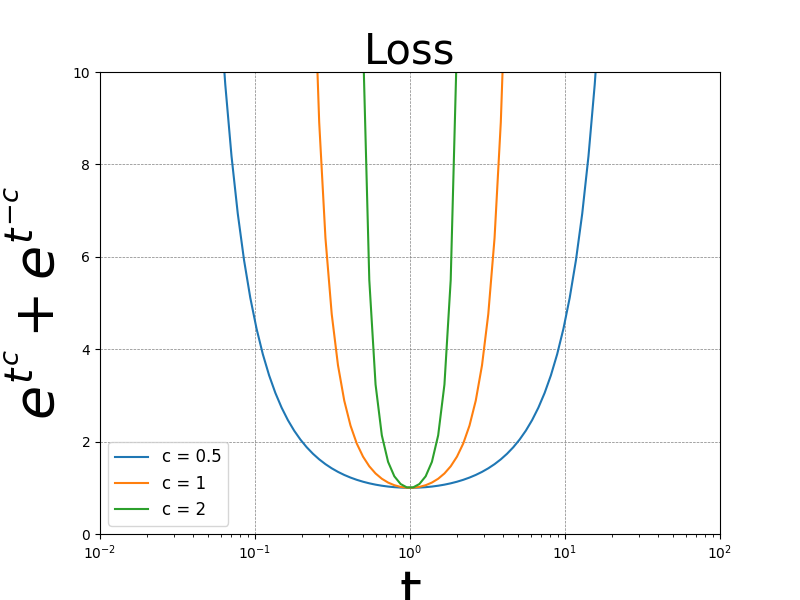
\includegraphics[width=\textwidth]{../figures/Figure_1b.png}
        \caption{Ground truth loss scaling function $g$ as a function of $t$}
        \label{fig:gt_loss}
    \end{minipage}
    \begin{minipage}{0.32\textwidth}
        \centering
        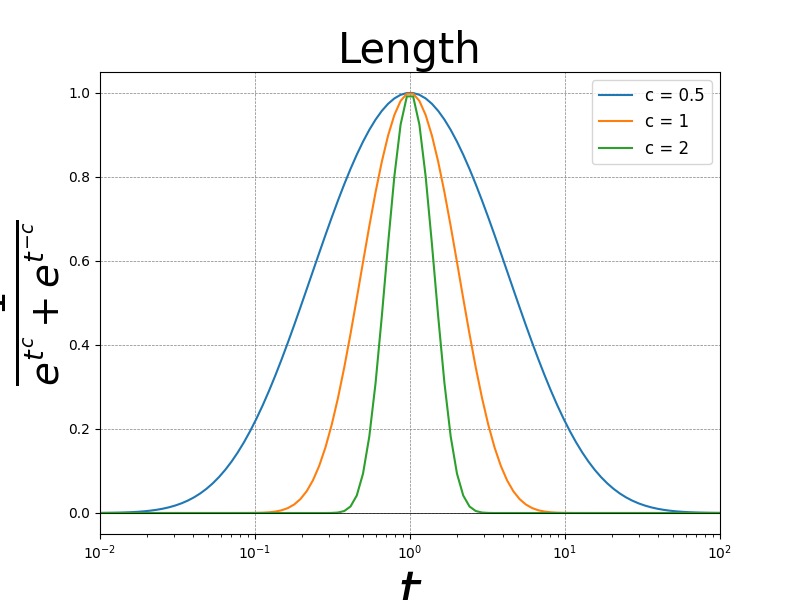
\includegraphics[width=\textwidth]{../figures/Figure_1a.png}
        \caption{Length as a function of $t$}
        \label{fig:length}
    \end{minipage}
    \begin{minipage}{0.32\textwidth}
        \centering
        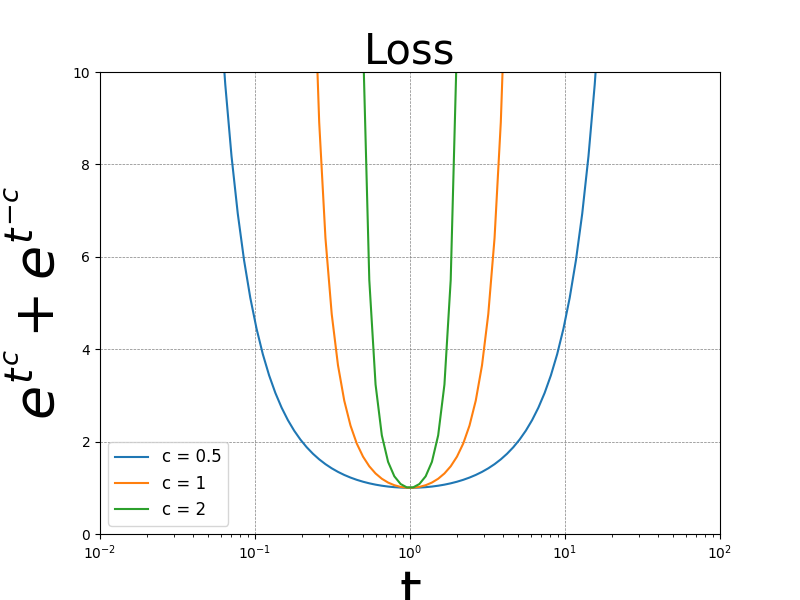
\includegraphics[width=\textwidth]{../figures/Figure_1b.png}
        \caption{Basis pursuit losses as a function of $t$}
        \label{fig:loss}
    \end{minipage}
    \caption{Plots of Length and Loss for different values of $c$.
    Since $t$ is one dimensional and therefore diagonalizable, basis pursuit and ground truth give identical loss values.}
    \label{fig:results}
\end{figure}

\subsection{Isometry pursuit}

We will show how to use an appropriate normalized matrix $w(\mathcal X)$ in multitask basis pursuit to identify submatrices of $\mathcal X$ that are as unitary as possible.
Multitask basis pursuit is a method for identifying sparse signals from overcomplete dictionaries, and the intuition behind its application in our setting is that submatrices consisting of vectors which are closer to 1 in length and more orthogonal will have smaller loss.
In contrast to the typical statistical setting, these features correspond to individual observations in our diversification example, and basis vectors of data manifold tangent spaces in our non-linear dimension reduction example.

Define the multitask basis pursuit penalty  % is this really a norm?
\begin{align}
\label{eq:bp}
\| \cdot \|_{1,2}: \mathbb R^{P \times D} &\to \mathbb R^+ \\ 
\beta &\mapsto  \sum_{p=1}^P  \|\beta_{p.}\|_2.
\end{align}
The isometry pursuit program is then
\begin{align}
\label{prog:isometry_pursuit}
\widehat \beta^{P}_c (\mathcal X)  := \arg \min_{\beta \in \mathbb R^{P \times D}} \| \beta \|_{1,2} \; : \; I_D = w ({ \mathcal X}, c) \beta.
\end{align}
The recovered functions are the indices of the dictionary elements with non-zero coefficients.
That is, they are given by $S(\beta)$ where 
\begin{align}
S: \mathbb{R}^{p \times d} &\to \binom{[P]}{d} \\
\beta &\mapsto \left\{ p \in [P] :  \|\beta_{p.}\| > 0 \right\}
\end{align}
and $\binom{[P]}{d} = \left\{ A \subseteq [P] : \left|A\right| = d \right\}$. 
\begin{algorithm}[H]
\caption{\isometrypursuit(Matrix $\mathcal X \in \mathbb R^{D\times P}$, scaling constant $c$)}
\begin{algorithmic}[1]
\STATE {\bf Output} $\widehat S= S (\widehat \beta_P(w_c(\mathcal X))$ 
\end{algorithmic}
\end{algorithm}

A key theoretical assertion for the feasibility of \isometrypursuit~ is that it is invariant to choice of basis for $\mathcal X$.
\begin{proposition}[Basis pursuit selection invariance]
\label{prop:basis_pursuit_selection_invariance}
Let $U \in \mathbb R^{D \times D}$ be unitary.
 Then $S(\widehat \beta  (U \mathcal X)) = S(\widehat \beta (\mathcal X))$.
\end{proposition}
A proof is given in Section \ref{proof:basis_pursuit_program_invariance}
This fact has as an immediate corollary that we may replace $I_D$ in the constraint by any unitary $D \times D$ matrix.
With these preliminaries, we may state our main result.
\begin{proposition}[Unitary selection]
\label{prop:unitary_selection}
Given a matrix $\mathcal X \in \mathbb R^{D \times P}$ with a rank $D$ submatrix $\mathcal X_{.\mathcal S} \in \mathbb R^{D \times D}$ that is unitary, $\mathcal S = S(\widehat{\beta} (\mathcal X)))$
 \end{proposition}
 
This proof admits two immediate generalizations.
First, any normalization function that satisfies the normalization conditions will do.
Second, assuming that we do in fact use $w$ for normalization, the ground truth and convex losses are equivalent for diagonalizable matrices.
This is summarized in the following proposition, which is slightly stronger than Proposition \ref{prop:unitary_selection}
 \begin{proposition}[Loss equivalence]
 Given a diagonalizable matrix $\mathcal X \in \mathbb R^{D \times D}$, $\|\widehat \beta_c^P(\mathcal X)\|_{1,2} = l_c (\mathcal X)$.
 \end{proposition}
This proposition should be thought of as applying to $D$ column matrices after selection.
We know that unitary submatrices minimize loss, and should they be present, they will be selected by either method. % Note (Sam): still need to prove!
This proposition shows that should diagonalizable matrices be selected, they will also have equivalent loss, but not necessarily that they will be selected.
% NOTE (Sam) is it just generally required that q(v) = g^{-1} (\|v\|) v/\|v\| basically?  Might need to make normalization notation more clear to state general proposition.

\subsection{Isometric lasso}

The convex loss function \ref{eq:bp} and linear constraint in \ref{prog:isometry_pursuit} admit a Lagrangian dual which we shall call Isometric Lasso.
While we defer full discussion of computational complexity to Section \ref{sec:computational_complexity}, the general principal which motivates the use of this formulation in our setting is the increased computational expediency in high-dimensions.

The Isometric Lasso loss is
\begin{align}
l_\lambda (\mathcal X, \beta) =  \|I_D -  \tilde{ \mathcal X}_c \beta\|_2^2 +  \lambda \| \beta \|_{1,2}
\end{align}
which can be optimized as
\begin{align}
\label{prog:isometric_lasso}
\hat {\beta_{\lambda}} (\mathcal X) = \arg \min_{\beta \in \mathbb R^{P \times D}} l_\lambda (\mathcal X, \beta)
\end{align}

Similarly to Section \ref{sec:isometry_pursuit}, we assert that $S(\widehat {\beta}_{\lambda} (\mathcal X))$.

\begin{proposition}[Lasso selection equivalence]
\label{prop:lasso_selection_equivalence}
Let $U \in \mathbb R^{D \times D}$ be unitary.
 Then $S(\widehat \beta_{\lambda}  (U \mathcal X)) = S(\widehat \beta_{\lambda} (\mathcal X))$.
\end{proposition}

This also covers changing the target variable.

Note that it also may be possible to argue the basis pursuit invariance from the lasso ones plus Lagranian duality, but to avoid taking the limit we prove both propositions  independently.

\subsection{Extension to non-linear spaces}

% NOTE (Sam): just use projected jacobian as argument to isometry pursuit.

\begin{proposition}[Isometry at a point selection]
\label{prop:local_isometry}
Given a set of functions $G$ that contains a subset that defines a locally isometric embedding at a point $\xi$, then these will be selected as $\arg \min_\beta$.
\end{proposition}
A proof is given in Section \ref{sec:local_isometry_proof}.

\subsection{Two-stage isometry pursuit}

A standard approach in the lasso literature is to first use the lasso to prune, prior to a final feature selection step.
This avoids issues from shrinkage caused by the lasso estimator at high values of $\lambda$.
For example, we cannot as of yet prove analogs of Proposition \ref{prop:unitary_selection} for the Lasso formulation, and similar lasso-specific conditions such as those found in \cite{Koelle2024-no} are not satisfied by overcomplete dictionaries.

\subsection{Implementation}

We use the multitask lasso from sklearn and the cvxpy package for basis pursuit.
We use the SCS interior point solver from CVXPY, which is able to push sparse values arbitrarily close to 0 \cite{cvxpy_sparse_solution}.
Data is IRIS and Wine, as well as flat torus from ldle.

\subsection{Computational complexity}
\label{sec:computation_complexity}

\section{Experiments}
\label{sec:experiments}

Say you are hosting an elegant dinner party, and wish to select a balanced set of wines for drinking and flowers for decoration.
We demonstrate \tsip~ and \greedy~ on the Iris and Wine datasets \citep{misc_iris_53, misc_wine_109, scikit-learn}.
This has an intuitive interpretation as selecting diverse elements that reflects the peculiar structure of the diversification problem.
Features like \textit{ petal width} are rows in $X$.
They are features on the basis of which we may select among the flowers those which are most distinct from another.
Thus, in diversification, $P = n$.

%add description of words
\begin{figure}[t]
   \centering
    % Row 1: Wine and Iris
    \begin{subfigure}[b]{0.45\textwidth}
        \centering
        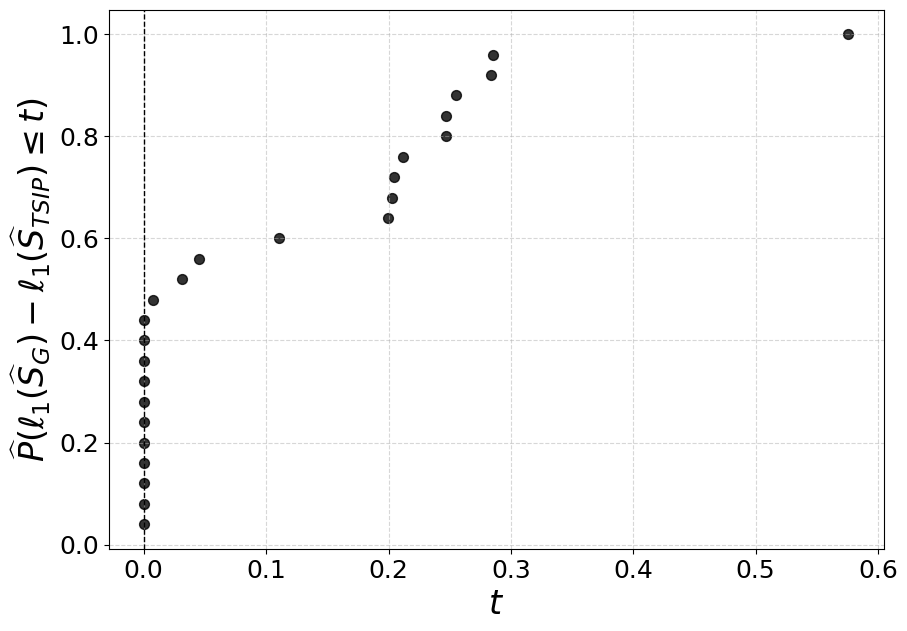
\includegraphics[width=\textwidth]{../figures/wine_standardized_isometry_losses_ecdf}
        \caption{Wine}
        \label{fig:wine_isometry_losses}
    \end{subfigure}
    \hfill
    \begin{subfigure}[b]{0.45\textwidth}
        \centering
        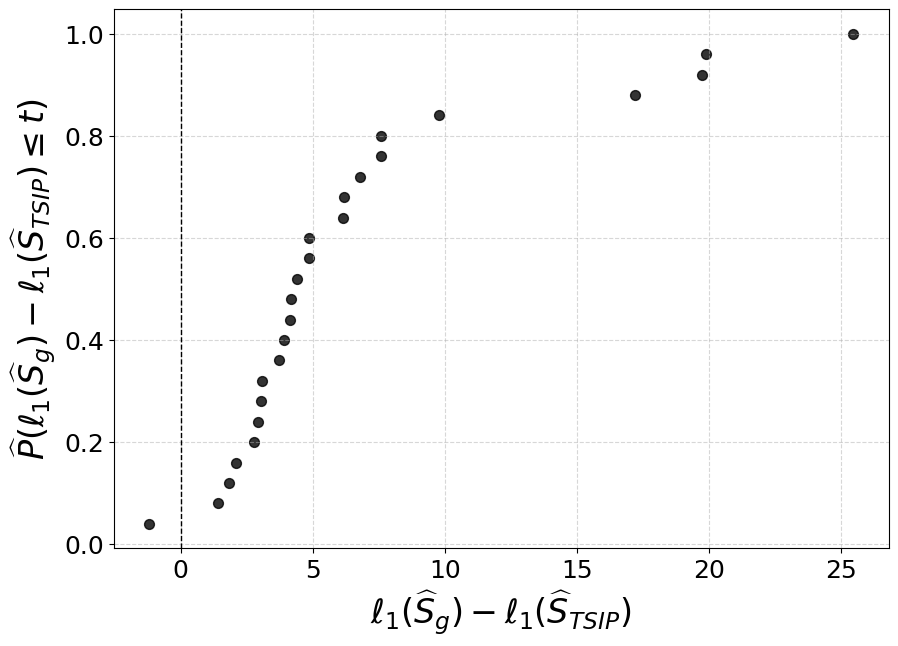
\includegraphics[width=\textwidth]{../figures/iris_standardized_isometry_losses_ecdf}
        \caption{Iris}
        \label{fig:iris_isometry_losses}
    \end{subfigure}

    \vspace{1em}

    % Row 2: Ethanol and Words
    \begin{subfigure}[b]{0.45\textwidth}
        \centering
        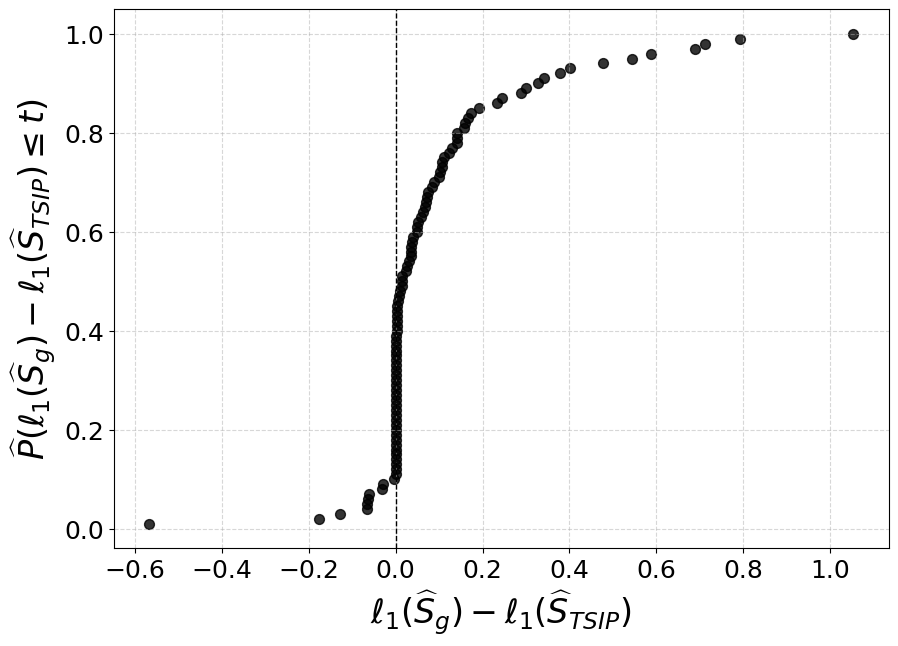
\includegraphics[width=\textwidth]{../figures/ethanol_isometry_losses_ecdf}
        \caption{Ethanol}
        \label{fig:ethanol_isometry_losses}
    \end{subfigure}
    \hfill
    \begin{subfigure}[b]{0.45\textwidth}
        \centering
        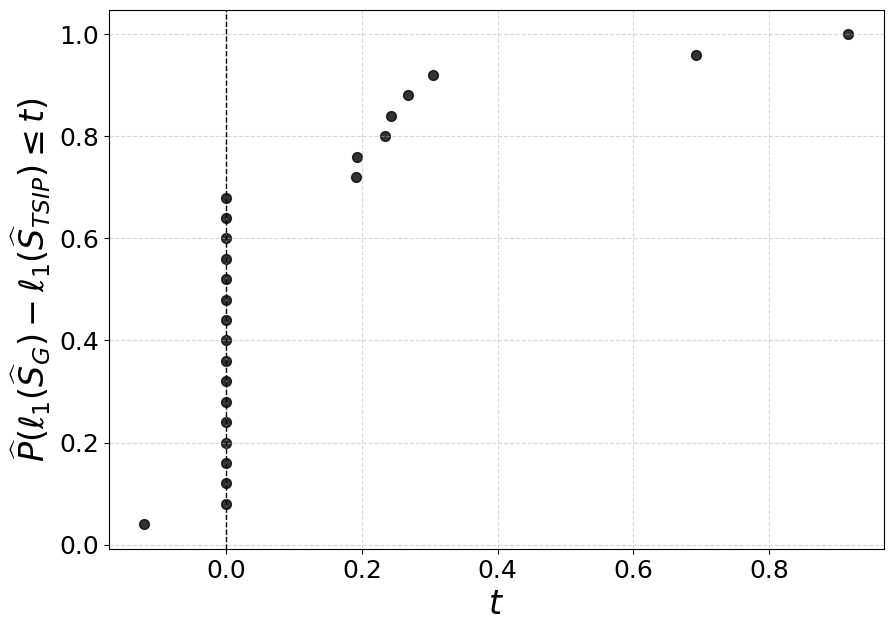
\includegraphics[width=\textwidth]{../figures/words_ecdf}
        \caption{Words}
        \label{fig:words_isometry_losses}
    \end{subfigure}
    \caption{Empirical CDFs of isometry losses $\ell_1(\widehat{S}_g) - \ell_1(\widehat{S}_{TSIP})$ for Wine, Iris, and Ethanol datasets across $R$ replicates.
    The CDF reflects the proportion of replicates where the greedy loss is less than or equal to the two-stage loss.
    As detailed in Table \ref{tab:experiments}, losses are generally lower for two-stage isometry pursuit solutions.}
    \label{fig:isometry_losses}
\end{figure}

We also analyze the Ethanol dataset from \citet{Chmiela2018-at, Koelle2022-ju}, but rather than selecting between bourbon and scotch we evaluate a dictionary of interpretable features  - bond torsions - for their ability to parameterize the molecular configuration space.
In this interpretability use case, columns denote gradients of informative features.
We compute Jacoban matrices of putative parametrization functions and project them onto estimated tangent spaces (see \citet{Koelle2022-ju} for preprocessing details).
Rather than selecting between data points, we are selecting between functions which parameterize the data.
This dataset exemplifies our motivating example - the search for locally isometric embeddings.

Finally, we also construct a small word embedding dataset.
Inspired by the linear representation hypothesis \citep{Park2023-hq,Mikolov2013-lt } and the construction over complete dictionaries of concepts in representation space, we apply isometric pursuit to prune down embeddings of concept dictionaries into their basis components.
As with the other datasets, we measure success primarily numerically against the ground truth objective values obtained by greedy solutions.

\begin{table}[h!]
\tiny
\centering
\begin{tabular}{|c|c|c|c|c|c|c|c|c|c|c|}
\toprule
Name & $D$ & $P$ & $R$ & $c$ & $\ell_1(X_{.\widehat{S}_{G}})$ & $|\widehat{S}|$ & $\ell_1(X_{.\widehat{S}})$ &
\begin{tabular}{c}
$\widehat P (\ell_1(X_{.\widehat{S}_{G}}) >$ \\
$\ell_1(X_{.\widehat{S}}))$
\end{tabular} &
\begin{tabular}{c}
$\widehat P (\ell_1(X_{.\widehat{S}_{G}}) =$ \\
$\ell_1(X_{.\widehat{S}}))$
\end{tabular} &
\begin{tabular}{c}
$\widehat P(\bar{\ell}_1(X_{.\widehat{S}_{G}}) >$ \\
$\bar{\ell}_1(X_{.\widehat{S}}))$
\end{tabular} \\
\midrule
Iris & 4 & 75 & 25 & 1 & 14 ± 7.3 & 6.7 ± 1 & 6.9 ± 1.4 & 0.96 & 0 & 2.4e-05 \\
Wine & 6 & 89 & 25 & 1 & 7.7 ± 0.33 & 13 ± 1.5 & 7.6 ± 0.29 & 0.64 & 0.16 & 6.3e-04 \\
Ethanol & 2 & 756 & 100 & 1 & 2.6 ± 0.3 & 90 ± 1.7e+02 & 2.5 ± 0.2 & 0.66 & 0.17 & 2.1e-05 \\
Words & 6 & 61 & 25 & 1 & 14 ± 1.3 & 11 ± 1.3 & 14 ± 1.2 & 0.52 & 0.12 & 2.1e-02 \\
\bottomrule
\end{tabular}
\caption{Experimental parameters and results.
For Iris and Wine, $\widehat P$ estimates result from random downsampling by a factor of $2$ to create $R$ replicates.
Distributional probabilities $\widehat P (\ell_1(X_{.\widehat{S}_{G}}) > \ell_1(X_{.\widehat{S}_{TSIP}}))$ and $\widehat P (\ell_1(X_{.\widehat{S}_{G}}) = \ell_1(X_{.\widehat{S}_{TSIP}}))$ are empirical across replicates, while asymptotic probabilities $\widehat P(\bar{\ell}_1(X_{.\widehat{S}_{G}}) > \bar{\ell}_1(X_{.\widehat{S}_{TSIP}}))$ is computed by paired two-sample T-test on  $\ell_1(X_{.\widehat S})$ and $\ell_1(X_{.\widehat S_{G}})$.
For brevity, in this table $\widehat S := \widehat {S}_{TSIP}$.
}
\label{tab:experiments}
\end{table}

For basis pursuit, we use the SCS interior point solver \citep{ocpb:16} from CVXPY \citep{diamond2016cvxpy, agrawal2018rewriting}, which is able to push sparse values arbitrarily close to 0 \citep{cvxpy_sparse_solution}.
Statistical replicas for Wine, Iris, and Words are created by resampling across $[P]$.
Due to differences in scales between rows, these are first standardized.
For the Wine dataset, even \brute~ on $\widehat {S}_{IP}$ is prohibitive in $D=13$, and so we truncate our inputs to $D=6$.
For Ethanol, replicas are created by sampling from data points and their corresponding tangent spaces are estimated in $B = 252$.

Figure \ref{fig:isometry_losses} and Table \ref{tab:experiments} show that the $\ell_1$ accrued by the subset $\widehat S_{G}$ estimated using \greedy~ with objective $\ell_1$ is higher than that for the subset estimated by \tsip.
This effect is statistically significant, but varies across datapoints and datasets.
Generally speaking, the ground truth loss obtained by greedy solutions is greater than obtained by two-stage Isometry Pursuit.
Figure \ref{fig:support_cardinalities} details intermediate support recovery cardinalities from \isometrypursuit.
We also evaluated second stage \brute~ selection after random selection of $\widehat S_{IP}$ but do not report it since it often lead to catastrophic failure to satisfy the basis pursuit constraint.
Wall-clock runtimes are given in Section \ref{sec:timing}.

Finally, we also analyze robustness of two-stage Isometry Pursuit to different choices of $c$ and $D$ on the Wine dataset in Figure \ref{fig:stacked_power_comparison}.
These show that the preference for the two-stage Isometry Pursuit solution is strongest around $c=1$ and is consistent across feature truncation dimensions.

\clearpage

\begin{figure}[t!]
    \centering
    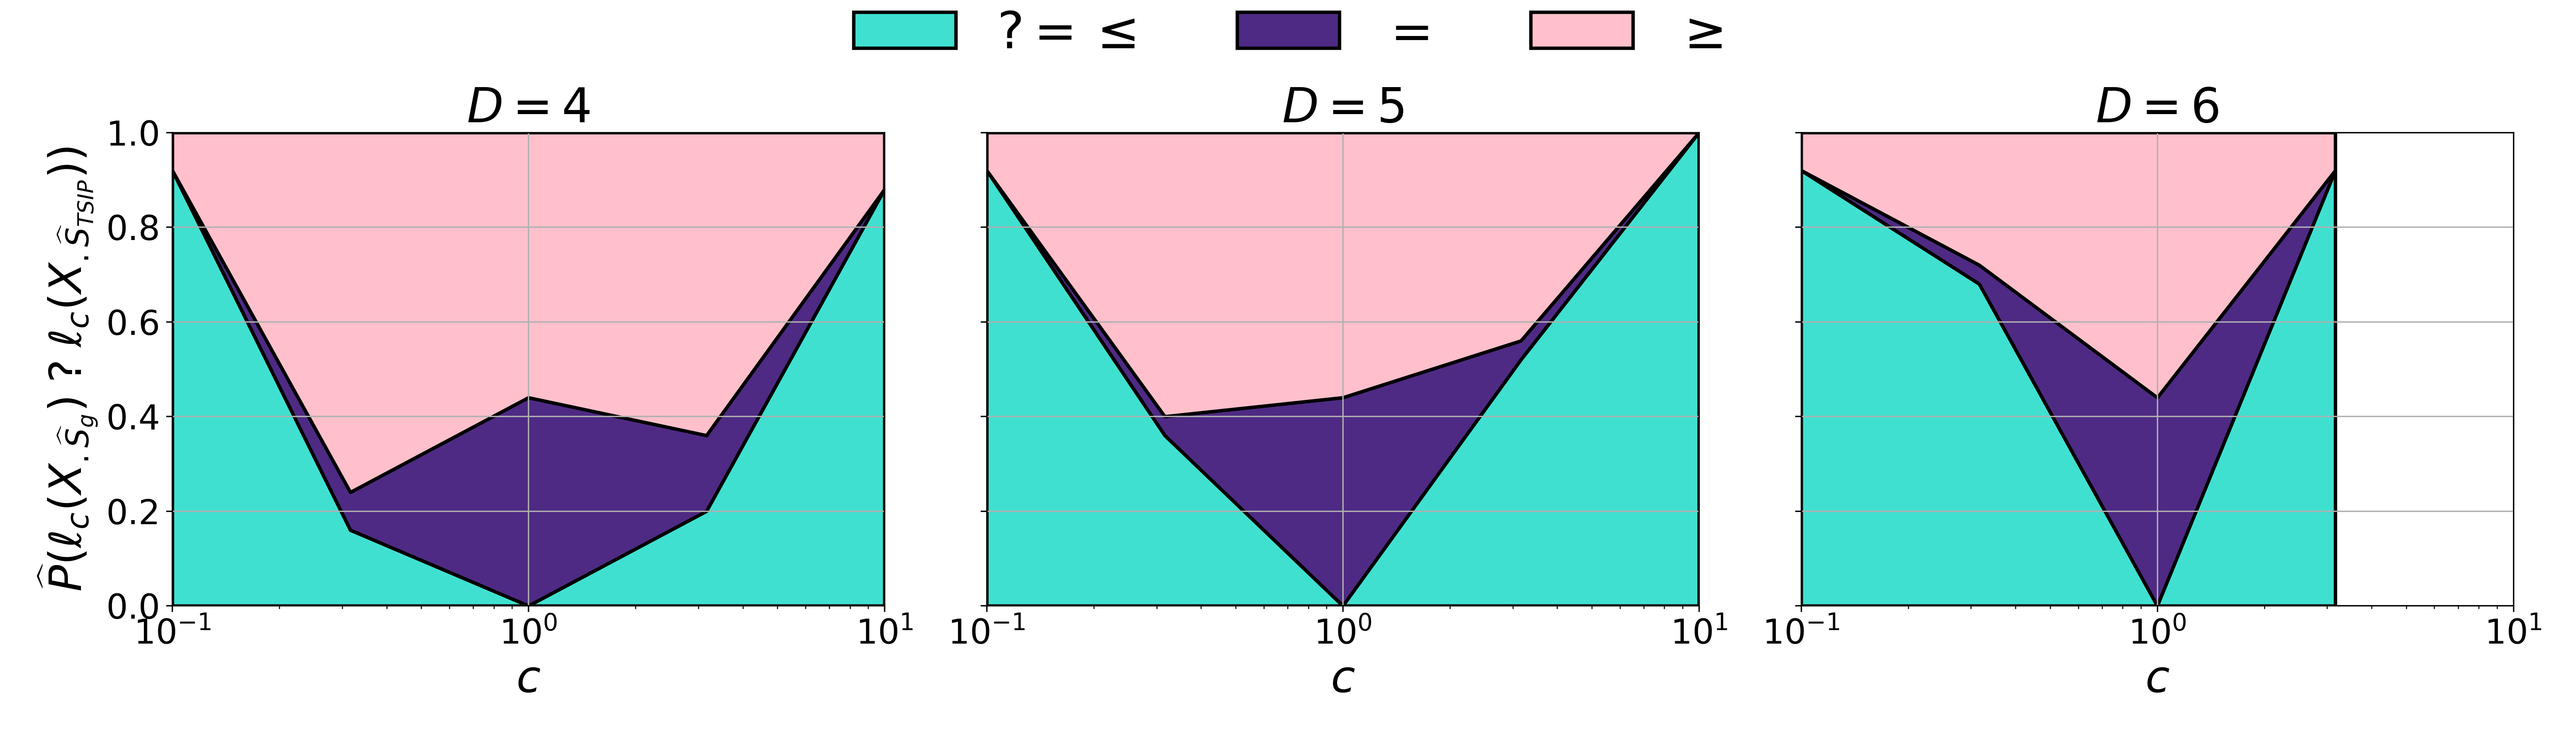
\includegraphics[width=\textwidth]{../figures/grid_power_comparison_filled.png}
    \caption{
        Proportions of support selection outcomes as power parameter $c$ varies, for different values of $D$ in the Wine dataset across various values of $c$.
        The turquoise area indicates when greedy solution  $\widehat{S}_G$ outperforms $\widehat{S}_{\text{TSIP}}$, gray shows ties, and pink indicates $\widehat{S}_{\text{TSIP}}$ is better.
        Solution at $c=10$ is not plotted for $D=6$ due to numerical overflow.
    }
    \label{fig:stacked_power_comparison}
\end{figure}




\section{Discussion}
\label{sec:discussion}

We have shown that multitask basis pursuit can help select isometric submatrices from appropriately normalized wide-matrices.
This approach - \isometrypursuit~ - is convex alternative to greedy methods for selection of orthonormalized features from within a dictionary.
\isometrypursuit~ can be applied to diversification and geometrically-faithful coordinate estimation.
Our experiments exemplify these applications, but more can be done.
One potential application is diversification in recommendation systems \cite{Carbonell2017-gi, Wu2019-uk, Langchain} and other retrieval systems such as in RAG \cite{Gao2023-cn, Pickett2024-ad, In2024-um, Weiss2024-xm, Vectara}.
Another is decomposing interpretable yet overcomplete dictionaries in transformer residual streams, with each token considered as generating its own tangent space.

Compared with the greedy algorithms used in such areas \cite{Carbonell1998-ji, Barioni, Drosou, Qin2012-ok, KUNAVER2017154, Guo-shengbo, Abdool,Yu2016AGA,  Huang2024-wr, Pickett2024-ad}, the convex reformulation may add speed and convergence to a global minima.
The comparison of greedy \cite{Mallat93-wi, Mallat, Pati-93, Tropp05-ml} and convex \cite{Chen2001-hh, Tropp06-sg,Chen2006TheoreticalRO} basis pursuit formulations has a rich history, and theoretical understanding of the behavior of this approximation is evolving.
Diversification problems have been cited as NP-hard, and isometry pursuit can be considered analogous to them in the sense of basis pursuit and the lasso against best subset selection, with the caveat that best subset selection of the basis pursuit loss minimizer isn't totally equivalent to isometry pursuit even though they share the same unique optimum.
Characterization of solutions resulting from removal of the restriction $|S| = D$ on the conditions of Proposition \ref{prop:unitary_selection} may help justify the second selection step.
That the solution of a lasso problem can sometimes be a non-singleton convex set containing the $\ell 0 $ solution is well-known \cite{Osborne2000OnTL, DOSSAL2012117, Chrtien2011OnTG, Tibshirani2012TheLP, Ewald2017OnTD, Ali2018TheGL, Schneider2020-qt, Mishkin2022TheSP,Dupuis2019TheGO,Debarre2020OnTU,Everink2024TheGA}, and it appears empirically in our situation that this can occur even when the design matrix is not in so-called general position.
The best subset support estimate - the isometry estimate - may be contained within the loss preimage fiber at the minimum loss.
The convergence of SCS algorithm to the 2 norm minimizing solution due to the dual constraint penalty and the convexity of this premise may then imply that the two stage procedure would then always succeed.
Related conditions have been discussed in \cite{Donoho2006ForML, Mishkin2022TheSP}, and we examine this topic experimentally in Section \ref{sec:deep_dive}.

Algorithmic variants include the multitask lasso \cite{ Hastie2015-qa} extension of our estimator, as well as characterization of $D$ function selection within spaces larger than $\mathbb R^D$.
Tangent-space specific variants have been studied in more detail in \cite{Koelle2022-ju, Koelle2024-no} with additional grouping across datapoints, and a corresponding variant of the isometry theorem that missed non-uniqueness was claimed in \cite{Koelle2022-lp}.
Comparison of our loss with curvature - whose presence prohibits $D$ element isometry - could prove fertile, as could comparison with the so-called restricted isometry property used to show guaranteed recovery at fast convergence rates in supervised learning \cite{Candes2005-dd, Hastie2015-qa}.

\newpage

\bibliography{ref}

\newpage

\section{Supplement}

This section contains algorithms and proofs in support of the main text.

\subsection{Algorithms}
\label{sec:algorithms}

We give definitions of the brute and greedy algorithms used in this paper.

\begin{algorithm}[H]
\caption{\brute(Matrix $\mathcal{X} \in \mathbb{R}^{D \times P}$, objective $f$)}
\begin{algorithmic}[1]
\FOR{each combination $S \subseteq \{1, 2, \dots, P\}$ with $|S| = D$}
    \STATE Evaluate $f(\mathcal{X}_{.S})$
\ENDFOR
\STATE {\bf Output} the combination $S^*$ that minimizes $f(\mathcal{X}_{.S})$
\end{algorithmic}
\end{algorithm}

\begin{algorithm}[H]
\caption{\greedy(Matrix $\mathcal{X} \in \mathbb{R}^{D \times P}$, objective $f$, selected set $S = \emptyset$, current size $d=0$)}
\begin{algorithmic}[1]
\IF{$d = D$}
    \STATE {\bf Return} $S$
\ELSE
    \STATE {\bf Initialize} $S_{\text{best}} = S$
    \STATE {\bf Initialize} $f_{\text{best}} = \infty$
    \FOR{each $p \in \{1, 2, \dots, P\} \setminus S$}
        \STATE {\bf Evaluate} $f(\mathcal{X}_{.(S \cup \{p\})})$
        \IF{$f(\mathcal{X}_{.(S \cup \{p\})}) < f_{\text{best}}$}
            \STATE {\bf Update} $S_{\text{best}} = S \cup \{p\}$
            \STATE {\bf Update} $f_{\text{best}} = f(\mathcal{X}_{.(S \cup \{p\})})$
        \ENDIF
    \ENDFOR
    \STATE {\bf Return} \texttt{Greedy}($\mathcal{X}$, $f$, $S_{\text{best}}$, $d+1$)
\ENDIF
\end{algorithmic}
\end{algorithm}

\subsection{Proofs}
\label{sec:proofs}

\subsubsection{Proof of Proposition \ref{prop:basis_pursuit_selection_invariance}}
\label{proof:basis_pursuit_program_invariance}

In this proof we first show that the penalty $\|\beta\|_{1,2}$ is unchanged by unitary transformation of $\beta$.

 \begin{proposition}{Loss equivalence}
 \label{prop:basis_pursuit_loss_equivalence}
 Let $U \in \mathbb R^{D \times D}$ be unitary.
 Then $\|\beta\|_{1,2} = \|\beta U \|$.
\end{proposition}

\begin{proof}
\begin{align}
\|\beta U \|_{1,2} &= \sum_{p = 1}^P \| \beta_{p.} U \| \\
&= \sum_{p = 1}^P \| \beta_{p.} \| \\
&= \|\beta \|_{1,2}
\end{align}
\end{proof}

We then show that this implies that the resultant loss is unchanged by unitary transformation of $\mathcal X$.

\begin{proposition}
 \label{prop:basis_pursuit_loss_equivalence}
 Let $U \in \mathbb R^{D \times D}$ be unitary.
 Then $\widehat \beta  (U \mathcal X) = \widehat \beta  ( \mathcal X) U$.
\end{proposition}

\begin{proof}
\begin{align}
\widehat \beta  (U \mathcal X)  &= \arg \min_{\beta \in \mathbb R^{P \times D}} \|\beta\|_{1,2}  \; : \; I_{D} = U X \beta \\
&= \arg \min_{\beta \in \mathbb R^{P \times D}} \|\beta\|_{1,2}  \; : \; U^{-1} U = U^{-1} U X \beta U \\
&= \arg \min_{\beta \in \mathbb R^{P \times D}} \|\beta\|_{1,2}  \; : \;  I_D = X \beta U \\
&= \arg \min_{\beta \in \mathbb R^{P \times D}} \|\beta U \|_{1,2}  \; : \;  I_D = X \beta U \\
&= \arg \min_{\beta \in \mathbb R^{P \times D}} \|\beta \|_{1,2}  \; : \;  I_D = X \beta.
\end{align}
\end{proof}


\subsubsection{Proof of Proposition \ref{prop:unitary_selection}}
\label{sec:local_isometry_proof}

 \begin{proposition}[Unitary selection]
\label{prop:generalized_unitary_selection}
Let $w_c$ be a normalization satisfying the conditions in Definition \ref{eq:symmetric_normalization}.  Then $\arg \min_{X_{.S} \in \mathbb R^{D \times D}} \widehat \beta^{D}_c (X_{.S}) $ is orthonormal.  Moreover when $X$ is orthonormal, $\min_{\beta \in \mathbb R^{P \times D}} \| \beta \|_{1,2} \; : \; I_D = w ( \mathcal X, c) \beta = D$.
 \end{proposition}
 
 \begin{proof}

The value of $D$ is clearly obtained by $\beta$ orthonormal, since by Proposition \ref{basis_pursuit_selection_invariance}, for $X$ orthogonal, without loss of generality 
\begin{align}
\beta_{dd'} = \begin{cases} 1 & d = d' \in \{ 1 \dots D\}  \\
0 & \text{otherwise}
\end{cases}.
\end{align}
Thus, we need to show that this is a lower bound on the obtained loss.

From the conditions in Definition \ref{eq:symmetric_normalization}, normalized matrices will consist of vectors of maximum length (i.e. $1$) if and only if the original matrix also consists of vectors of length $1$.
Such vectors will clearly result in lower basis pursuit loss, since longer vectors in $X$ require smaller corresponding covectors in $\beta$ to equal the same result.

Therefore, it remains to show that $X$ consisting of orthogonal vectors of length $1$ have lower compared with $X$ consisting of non-orthogonal vectors.
Invertible matrices $X_{.S}$ admit QR decompositions $\tilde X_{.S} = QR$ where $Q$ and $R$ are orthonormal and upper-triangular matrices, respectively \citep{Anderson1992-fb}.
Denoting $Q$ to be composed of basis vectors $[e^1 \dots e^d]$, the matrix $R$ has form
\begin{align}
R = \begin{bmatrix}
\langle e^1, X_{.S_1} \rangle & \langle e^1,  X_{.S_2} \rangle  &\dots &  \langle e^1,  X_{.S_D} \rangle \\
0 & \langle e^2,  X_{.S_2} \rangle & \dots  &  \langle e^2,  X_{.S_D} \rangle\\
0 & 0 & \dots & \dots  \\
0 & 0 & \dots & \langle e^d, X_{.S_D} \rangle 
\end{bmatrix}.
\end{align}
Thus, $|R_{dd} | \leq \|X_{.{S_{d}}}\|_2$, with equality obtained across $d$ only by orthonormal matrices.
On the other hand, by Proposition \ref{basis_pursuit_selection_invariance}, $l(X) = l(R)$ and so $\|\beta\|_{1,2} = \|R^{-1}\|_{1,2}$.
Since $R$ is upper triangular it has diagonal elements $\beta_{dd} = R_{dd}^{-1}$ and so $\|\beta_{d.}\| \geq \| X_{.{S_d}}\|^{-1} = 1$.
That is, the penalty accrued by a particular covector in $\beta$ is bounded from below by $1$ - the inverse of the length of the corresponding vector in $X_{.S}$ - with equality occurring only when $X_{.S}$ is orthonormal.


\end{proof}


\end{document}